\chapter{Implementación: Configuración} % Main chapter title

\label{Chapter5} 

%--------------------------------------------------------
\section{Configuración de HTCondor}

Se deben tener en claro dos cosa a la hora de configurar una máquina para el uso de HTCondor, si esta sera un nodo de trabajo, o sera el nodo maestro que se encarga de enviar las tareas que se llevaran a cabo.

Dado que este trabajo esta basado en un cluster oportunista, se centra en la configuración de los nodos que realizan los trabajos ("workers").

\subsection{Configuración inicial}

Una vez terminada la instalación de las dependencias necesarias, se procede con la creación y modificación del archivo que contendrá la configuración con la cual iniciará el nodo de trabajo. 

\textbf{Para tener en cuenta:} Los cambios que se realizan a continuación se hacen como usuario \textbf{root} que es quien tiene los permisos para modificar estos archivos.

Primero crearemos el archivo que contendrá la configuración en la ruta:

\textit{/etc/condor/config.d/}

y le colocaremos como nombre \textbf{spider.conf}

\textbf{cd /etc/condor/config.d/}

\textbf{touch spider.conf}

Abrimos el archivo \textbf{spider.conf} y procedemos a editarlo

\begin{lstlisting}
UID_DOMAIN = unitecnologica.edu.co
####################################################################
# Nombre legible para el Condor pool
COLLECTOR_NAME = "Mi cluster en $(UID_DOMAIN)"
# Permisos de escritura
ALLOW_WRITE = *.$(UID_DOMAIN)
CONDOR_ADMIN = root@$(FULL_HOSTNAME)
####################################################################
# The following should be the full name of the head node
CONDOR_HOST = 172.16.9.100
####################################################################
# Rango de puertos usados por condor 
# se deben abrir estos puertos en el firewall de ser necesario
IN_HIGHPORT = 9999
IN_LOWPORT = 9000
####################################################################
# This is to enforce password authentication
SEC_DAEMON_AUTHENTICATION = required
SEC_DAEMON_AUTHENTICATION_METHODS = password
SEC_CLIENT_AUTHENTICATION_METHODS = password,fs,gsi,kerberos
SEC_PASSWORD_FILE = /etc/condor/password
ALLOW_DAEMON = condor_pool@*
##  Sets how often the condor_negotiator starts a negotiation cycle
##  for negotiator and schedd).
#  Defined in seconds and defaults to 60 (1 minute), default is 300.
NEGOTIATOR_INTERVAL = 20
##  Scheduling parameters for the startd
TRUST_UID_DOMAIN = TRUE
####################################################################
# start as available and do not suspend, preempt or kill
START = True
SUSPEND = False
CONTINUE = False
PREEMPT = False
KILL = False
WANT_SUSPEND = True
WANT_VACATE = True
####################################################################
#Como es worker, solo debe iniciar dos demonios
DAEMON_LIST = MASTER, STARTD
SOFT_UID_DOMAIN = TRUE
\end{lstlisting} 


\subsection{Seguridad y autenticación}
Para el manejo de la seguridad en el envío de trabajos y como se comunican las maquinas se colocan los  parámetros, y se agrega la clave del nodo maestro, que es la clave del pool de máquinas.

Para ello, se reinicia el servicio de condor, y luego se ejecuta el siguiente comando

\begin{lstlisting}
condor_store_cred -c add
\end{lstlisting}
Para ingresar la clave previamente compartida del nodo maestro. 

\begin{figure}[h]
\centering
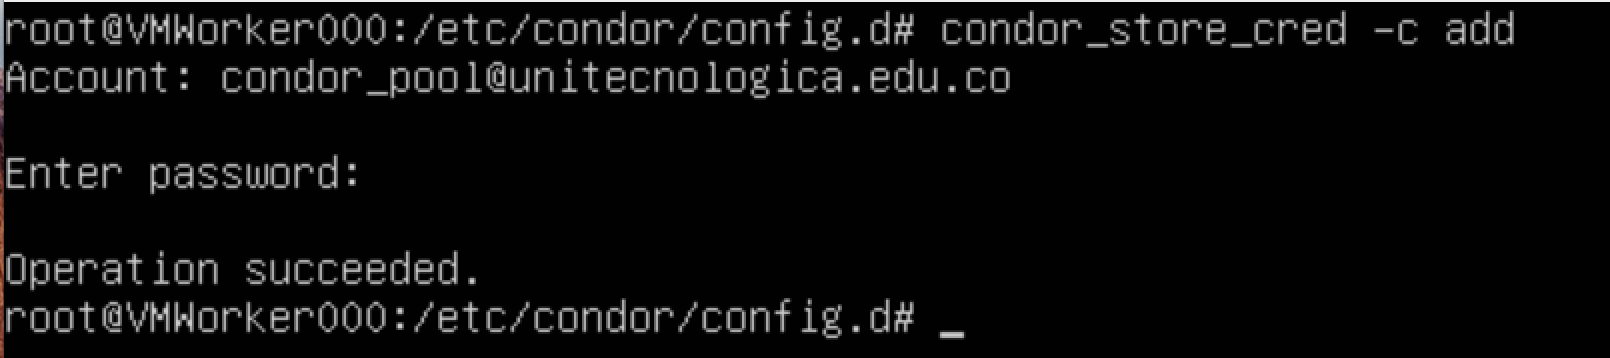
\includegraphics[width=0.8\textwidth]{Figures/pswrdok.png}
\decoRule
\caption{Contraseña compartida aceptada}
\label{fig:condor creed}
\end{figure}
\FloatBarrier

Vemos que la maquina ya lista sus recursos en el pool de condor, la captura fue tomada desde uno de los servidores físicos del plantel, que ya hace parte del cluster.

el comando para listar los recursos disponibles en el pool es:
\begin{lstlisting}
condor_status
\end{lstlisting}

\begin{figure}[h]
\centering
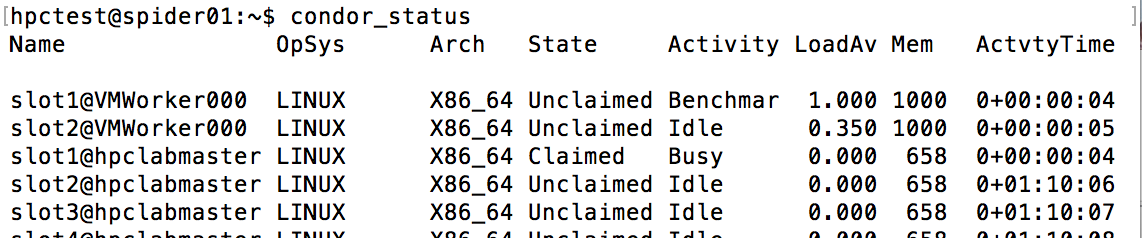
\includegraphics[width=0.9\textwidth]{Figures/vmwok.png}
\decoRule
\caption{Recursos de nuestra máquina en el pool}
\label{fig:condor creed}
\end{figure}
\FloatBarrier

\subsection{Configuración para Java}

Para poder usar el universo \textbf{Java}, no basta con tener el entorno de ejecución instalado, se debe descargar y configurar varios archivos, para que el nodo maestro \textbf{\textit{hpclabmaster}} pueda reconocer las máquinas que disponen de este entorno.

editamos el archivo: sources.list

\textbf{nano /etc/apt/sources.list}

y al final del mismo colocamos la linea siguiente:

\begin{figure}[h]
\centering

\includegraphics[width=1\textwidth]{Figures/sourceedit.png}
\decoRule
\caption{Repositorio fuente }
\label{fig:source}
\end{figure}
\FloatBarrier

Luego de esto descargamos la llave publica para HTCondor con el siguiente comando.

wget -qO - http://research.cs.wisc.edu/htcondor/debian/HTCondor-Release.gpg.key | sudo apt-key add -

Luego se descarga el archivo necesario para que htcondor reconozca y admita la máquina de trabajo como una que tiene el universo de Java disponible y habilitado. El archivo necesario para esto es : \textbf{\textit{scimark2lib.jar}}

nos movemos a la ruta: \textit{cd /usr/lib/condor/}

y allí ejecutamos el siguiente comando:

\textbf{wget http://math.nist.gov/scimark2/scimark2lib.jar}

Una vez descargado el archivo, se ejecutan los siguientes comandos, en orden para que condor reconozca los cambios realizados.

\textbf{apt update}

\textbf{apt dist-upgrade}

\textbf{apt install condor} (Este ultimo reinstala la herramienta para tomar los cambios realizados)

Reiniciamos el servicio HTCondor, y para confirmar que el universo java esta habilitado ejecutamos el comando :

\begin{lstlisting}
condor_status -java
\end{lstlisting} 
\begin{figure}[h]
\centering
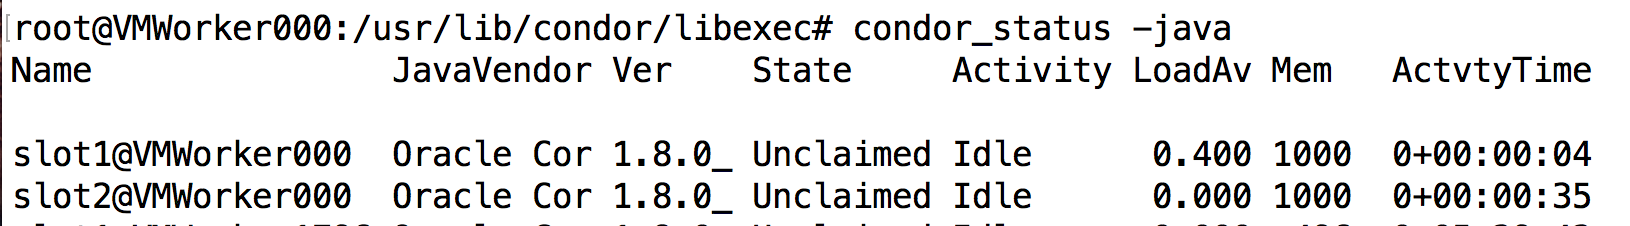
\includegraphics[width=1\textwidth]{Figures/javaready.png}
\decoRule
\caption{Universo Java Disponible }
\label{fig:Java Universe}
\end{figure}
\FloatBarrier

\textbf{NOTA:} Los pasos necesarios para el correcto funcionamiento del universo Java se realizan ya que en las nuevas distribuciones (versión 8.X en adelante) de la herramienta HTCondor no contienen el archivo de java necesario (\textbf{\textit{scimark2lib.jar}}) para que la herramienta reconozca las máquinas habilitadas con este universo.

Ahora la máquina esta lista para ser usada como nodo de trabajo en el cluster, en el apartado de pruebas se llevará a cabo una para mostrar la ejecución de trabajos en Java.


\section{Script adicional}

Como serán máquinas diferentes que tendrán los nodos de ejecución, es necesario diferenciarlas, para ello, se crea un script para bash para que cambie el nombre de la maquina en la primera ejecución de la misma, luego el script se elimina a si mismo evitando futuros cambios de nombre.

Para el nombre se usa el nombre seguido numero aleatorio , quedando de esta manera ejemplo \textit{VMWorker123456}

\begin{figure}[h]
\centering
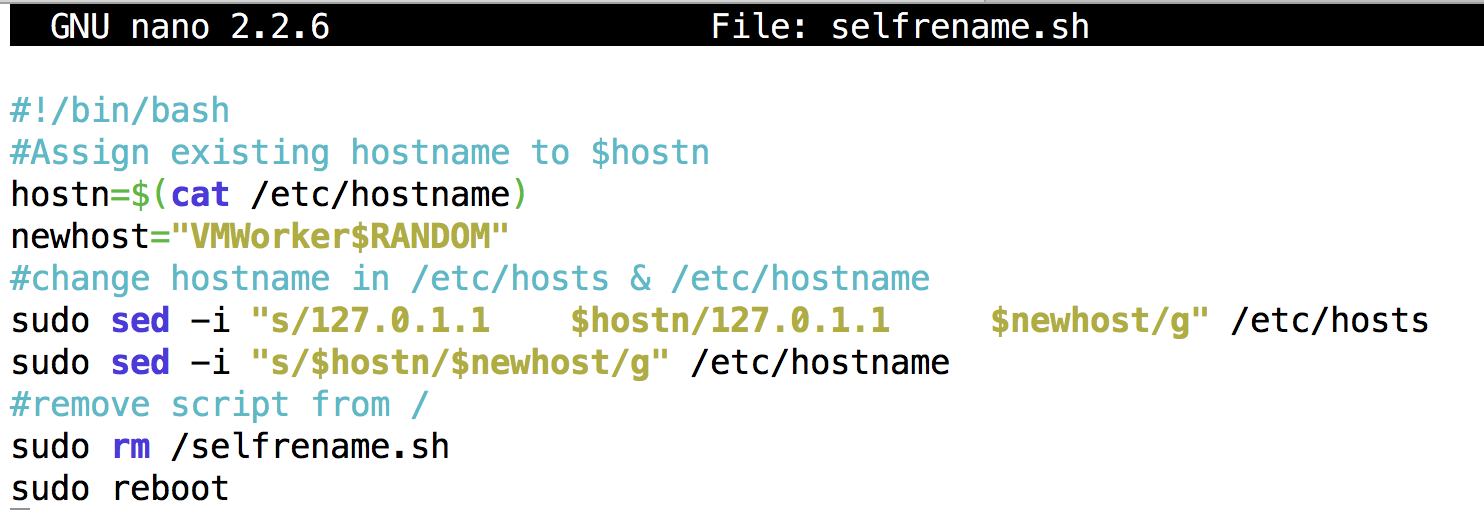
\includegraphics[width=1\textwidth]{Figures/scriptrename.png}
\decoRule
\caption{Script para renombrar la máquina }
\label{fig:rename script}
\end{figure}
\FloatBarrier

Este script modifica los archivos \textbf{\textit{hostname}} y \textbf{\textit{hosts}} que están en las rutas respectivas:

\textbf{\textit{/etc/hostname}} y \textbf{\textit{/etc/hosts}}

una vez creado el archivo, le damos permisos de ejecución con el comando:

\textbf{chmod a+x selfrename.sh}

luevo editamos el archivo \textit{rc.local} y agregamos el script para que se ejecute al iniciar la máquina.

\textbf{nano /etc/rc.local}

y al final colocamos la linea respectiva al script.

\begin{figure}[h]
\centering
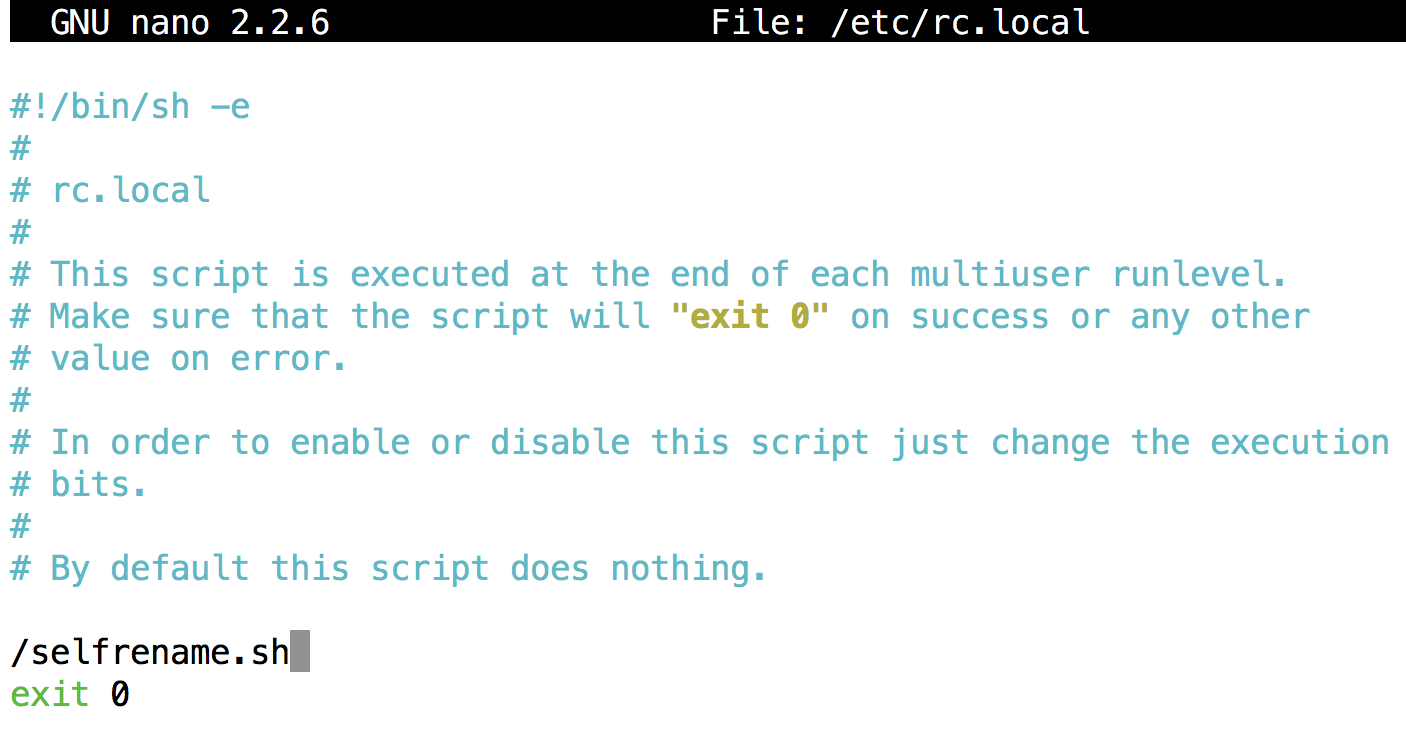
\includegraphics[width=1\textwidth]{Figures/rclocal.png}
\decoRule
\caption{Script para renombrar la máquina }
\label{fig:rename script}
\end{figure}
\FloatBarrier





%-----------------------------------------------------------------------------------------